%
% Capítulo 1
%
\chapter{Introdução} \label{cap:intro}
Um processo de averiguação inicia-se com a receção, por parte da CAPT, de um pedido submetido por um dos seus clientes, habitualmente seguradoras Estes pedidos contêm informação preliminar relativa ao sinistro, nomeadamente a localização da ocorrência, os intervenientes envolvidos, a data deste, entre outros elementos relevantes para a abertura do processo de averiguação.

Atualmente, os pedidos são recebidos de forma não uniforme, o que introduz dificuldades operacionais no tratamento e acompanhamento dos processos, o que obriga os colaboradores da CAPT a recorrer a procedimentos pouco padronizados. A inexistência de uma plataforma centralizada limita ainda a capacidade da gestão em obter uma visão global da operação e em tomar decisões informadas, o que pode originar situações de distribuição desequilibrada de carga de trabalho e incumprimento de prazos.

Após a receção de um pedido de averiguação, é necessário proceder à sua análise e atribuição de um averiguador e de um supervisor. O averiguador desloca-se ao local da ocorrência, realiza as diligências necessárias, recolhendo evidências relevantes e elabora um relatório técnico que contém toda a informação apurada durante o processo de investigação. Posteriormente, esse relatório é submetido para validação pelo supervisor, responsável por garantir que o conteúdo produzido cumpre os padrões de qualidade e conformidade definidos pela CAPT antes da sua entrega ao cliente final.

Com a implementação da plataforma IPW (\textit{Insurance Portal Workflow}), pretende-se criar um ambiente de trabalho mais estruturado, centralizado e normalizado, permitindo uma definição clara das responsabilidades de cada interveniente e promovendo uma maior rastreabilidade dos processos de averiguação.

Para suportar esta organização operacional, foram definidos cinco perfis distintos de utilizador:

\begin{itemize}
\item \textbf{Triador} — responsável pela receção dos pedidos de averiguação, criação de processos e pela sua atribuição aos averiguadores e supervisores;

\item \textbf{Averiguador} — responsável pela realização das investigações no terreno e pela elaboração do respetivo relatório técnico;

\item \textbf{Supervisor} — responsável pela validação dos relatórios técnicos produzidos pelos averiguadores de uma determinada área de especialização, como, por exemplo, sinistros automóveis ou acidentes de trabalho;

\item \textbf{Gestor} — responsável pela validação final dos relatórios aprovados pelos supervisores, assegurando um segundo nível de controlo e supervisão sobre as diferentes áreas operacionais da organização;

\item \textbf{Administrador} — responsável pela gestão da plataforma IPW, incluindo a criação de utilizadores, atribuição de perfis e gestão de permissões de acesso.

\end{itemize}

\begin{figure}[h]
\begin{center}
\resizebox{150mm}{!}{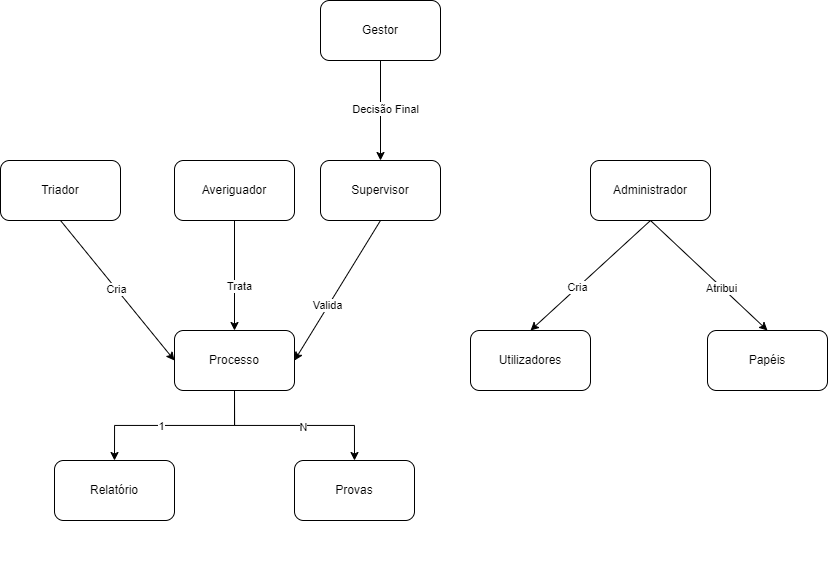
\includegraphics{./figures/Diagrama_blocos.png}}
\end{center}
\caption{Perfis de utilizadores da na plataforma IPW.}\label{fig:diagrama_blocos}
\end{figure}

\newpage
\section{Objetivos}
O presente projeto tem como principal objetivo o desenvolvimento da plataforma \textit{Web}, \textit{IPW} \textit{(Insurance Portal Workflow)}, para suporte à gestão de processos de averiguação de sinistros da CAPT Consulting. A solução pretende melhorar a organização operacional da empresa, promovendo maior uniformização de procedimentos, rastreabilidade da informação e capacidade de monitorização da atividade.

De forma mais específica, definiram-se os seguintes objetivos:

\begin{itemize}
\item Centralizar a informação relativa aos processos de averiguação numa única plataforma integrada;

\item Estruturar o processo de atribuição e acompanhamento de averiguações entre os diferentes intervenientes da organização;

\item Garantir o registo e rastreabilidade das interações realizadas ao longo do ciclo de vida de um processo;

\item Disponibilizar mecanismos de gestão documental associados aos processos de averiguação;

\item Fornecer indicadores operacionais e ferramentas de monitorização que suportem a supervisão e a tomada de decisão.

\end{itemize}

\newpage


\section{Estado da Arte}
\label{sec:estado_da_arte}

Existem diversas aplicações de \textit{workflow} e tecnologias de suporte disponíveis no mercado, de diferentes tipos. Fornecem uma variedade de recursos, padrões e funcionalidades para auxiliar a automação, segurança e otimização de fluxos de trabalho empresariais, dividindo-se nas seguintes categorias:

\begin{itemize}
    \item \textbf{Gestão de Processos e Dados Operacionais} -- Plataformas centralizadas permitem gerir a recepção e processamento uniforme de fluxos de trabalho que lidam com volumes crescentes de dados. O tratamento organizacional de informação em grande escala enquadra-se no conceito moderno de \textit{Big Data}, conforme definido formalmente pela \textit{Oracle}~\cite{oracle-bigdata}, exigindo a aplicação de técnicas fundamentais de extração e análise de conhecimento estruturado (\textit{data mining})~\cite{6547630}.
    
    \item \textbf{Arquitetura Web e Interface de Utilizador} -- No panorama de sistemas computacionais interligados através de redes rápidas~\cite{6824752}, o processamento de aplicações assenta nas bases lógicas fundamentais estabelecidas pelas arquiteturas computacionais clássicas~\cite{Neumann:1958:CB:578873}. A nível aplicacional, a engenharia contemporânea exige a utilização de estilos de programação limpos e modulares~\cite{Kernighan:1982:EPS:578130}, suportados por ecossistemas robustos de \textit{backend} como o \textit{Spring Boot}~\cite{spring-boot}. No ambiente de interface (\textit{frontend}), o desenvolvimento é enriquecido pela adoção de bibliotecas componentes visuais estandardizadas como o \textit{Material UI}~\cite{material-ui}, pela gestão dinâmica de feedback reativo através do \textit{notistack}~\cite{notistack}, e pelo suporte à internacionalização multi-idioma nativa via \textit{react-i18next}~\cite{react-i18next}.
    
    \item \textbf{Segurança e Controlo de Acessos} -- Mecanismos assentes no padrão de tokens digitais criptográficos constituem a base indispensável para a autenticação em APIs Web. A emissão, assinatura e validação segura de estruturas \textit{JSON Web Token} (JWT)~\cite{rfc-jwt} são garantidas tanto no servidor como no cliente através de módulos focados em encriptação como a biblioteca \textit{jose}~\cite{jose}. O ecossistema de segurança é consolidado através do framework \textit{Spring Security}~\cite{spring-security}, viabilizando a aplicação formal do modelo RBAC (\textit{Role-Based Access Control}) para restrição de rotas e funcionalidades por papéis operativos~\cite{nist-rbac}.
    
    \item \textbf{Persistência e Tradução de Dados} -- Sistemas de gestão de bases de dados garantem que as restrições de integridade transacional de um \textit{workflow} decorram sem condições de corrida. A otimização destes repositórios relacionais para buscas rápidas e indexação de metadados de utilizadores recorre a técnicas estruturadas de pesquisa aproximada em dicionários~\cite{Boytsov:2011:IMA:1963190.1963191}, mitigando também as restrições físicas de paginação no motor de persistência através de modelos eficientes de tradução de endereços virtuais em memória externa~\cite{Jurkiewicz:2015:MVA:2627368.2656337}.
\end{itemize}

Quanto à disponibilidade, licenciamento e custo destas soluções, o panorama varia substancialmente. Enquanto os ecossistemas de desenvolvimento e motores de persistência (\textit{Spring Boot, PostgreSQL, Material UI}) representam componentes de código aberto (\textit{open-source}) altamente robustos e livres de custos de licenciamento direto, as plataformas de \textit{workflow} verticais proprietárias de mercado exigem subscrições dispendiosas, calculadas muitas vezes pelo volume de utilizadores ou processos operacionais ativos.

Apesar da existência deste tipo de aplicação ser muito ampla no mercado, este projeto focou-se em desenvolver algo específico para a instituição, preservando algumas funcionalidades genéricas para possível implementação por outras instituições ou empresas. Além disso, para a correta implementação de um software de \textit{workflow} documental, a escolha no mercado seria ou muito ambígua, ou envolveria mais do que um fornecedor, visto que não foi encontrado software de \textit{workflow} de momento no mercado que fornecesse todas as funcionalidades previstas deste projeto numa única aplicação.
\section{Organização do documento}
